\documentclass[11pt,oneside]{scrbook}
\usepackage[a4paper,margin=2.4cm,marginparwidth=1.8cm,marginparsep=0.4cm]{geometry}
\usepackage{../common/rlstudy}
\usepackage[ruled,vlined]{algorithm2e}
\newcommand{\Reg}{\mathrm{Reg}}

\title{{\color{rlblue}\textbf{Week 11} \\ \Huge Contextual Bandits and Off-Policy Evaluation}}
\author{STUDY-RL --- a self-paced Deep RL curriculum}
\date{\today}

\begin{document}
\maketitle
\tableofcontents
\newpage

% ============================================================================
\chapter*{Learning objectives}
\addcontentsline{toc}{chapter}{Learning objectives}


% Teaching companion: a small example before the full lecture.
\noindent\textbf{Study companion.} Read \texttt{teaching\_guide.md} in this
folder for step-by-step examples, an analogy with its limits, and self-checks.
Then use \texttt{workbook.ipynb} to implement and vary the calculations.
\par\medskip

\begin{keyidea}
By the end of this lecture you will be able to:
\begin{enumerate}\setlength\itemsep{2pt}
  \item Derive the UCB1 regret bound sketch from Hoeffding and Lai--Robbins, and
        contrast it with KL-UCB, MOSS, and Thompson Sampling.
  \item Show that the LinUCB posterior mean is the closed-form ridge solution
        $\hat\theta_a = A_a^{-1} b_a$ with $A_a = \lambda I + \sum_t x_t x_t^\top$.
  \item Prove that Inverse Propensity Scoring (IPS) is unbiased, derive its
        variance, and explain why Self-Normalised IPS (SNIPS) is biased but
        often dominant in mean squared error.
  \item Derive the Doubly Robust estimator and prove its double-robustness:
        consistent if \emph{either} the propensity \emph{or} the reward model
        is correct.
  \item Build a synthetic synthetic insurance lead--broker contextual bandit (6 brokers,
        8 lead features), collect $\varepsilon$-greedy logs, and run SNIPS,
        Direct, DR, and SWITCH-DR against three counterfactual policies.
  \item Read off a bias/variance trade-off plot and pick $\tau$ for SWITCH.
  \item State the four production gotchas: logging propensities, overlap
        (positivity) failure, delayed feedback bias, and propensity overfitting.
\end{enumerate}
\end{keyidea}

% ============================================================================
\chapter{Motivation and intuition}

A \emph{bandit} is a Markov Decision Process collapsed to one step: at every
round you observe a context $x_t$, pick an arm $a_t \in \{1,\dots,K\}$, and
receive a noisy reward $r_t$. There is no transition; the next round's
context is independent of your action.\marginnote{Why bother with such a
small problem? Because almost every applied ML system is at heart a bandit
once the deep-learning fog clears: pick this ad / pick this thumbnail / pick
this broker.}

The puzzle is the same as in MDPs --- balance \emph{exploration} (try arms
whose value you do not know) with \emph{exploitation} (use the best arm you
have seen). What is gone is the credit-assignment chain. What is gained is
\textbf{a fully solvable, tightly characterised problem} where every
algorithmic trick (UCB, posterior sampling, importance sampling, doubly
robust estimation) has a clean derivation and a sharp regret bound. Master
this and the deeper RL material reduces to ``do this, but with a target
network and a replay buffer''.

\section{Two running examples}

\textbf{synthetic insurance lead-broker matching.} A motor-insurance comparator routes
each incoming \emph{lead} (a quote form) to one of $K$ brokers. The reward
is \emph{bind}: did the broker convert the lead into a sold policy?
Features include postcode band, vehicle power, prior claims, channel
(direct vs.\ aggregator), age band. The platform must (i) maximise binds,
(ii) keep brokers happy by sending them leads that match their book of
business, and (iii) audit the policy offline before pushing changes to
production. \emph{This is a contextual bandit with delayed, partially
observed feedback.}

\textbf{ATS candidate--job ranking.} (Treated in depth in Week 12.) A
recruiter platform must rank candidates for a requisition. The reward is
hire. Position bias makes naive click-modelling actively misleading. The
re-ranker is a contextual bandit on top of a two-tower retriever.

\section{Anchoring to what you already know}

If you know logistic regression, you know LinUCB --- it is logistic /
ridge regression with a confidence ellipsoid bolted on. If you know dropout
as a Bayesian approximation, you know Thompson Sampling --- it is posterior
sampling, but cheaper. If you know cross-validation, you know off-policy
evaluation --- it is the same idea: estimate held-out performance, but with
an importance-weight correction because the held-out set was generated by
a different policy.

\begin{pitfall}
Bandit literature is split between the \emph{stochastic} setting (rewards
i.i.d.\ given arm) and the \emph{adversarial} setting (rewards chosen by an
adversary). Almost everything in this chapter is stochastic. Production
matching is somewhere in between: brokers and recruiters are slow-moving
adversaries (incentive-compatibility) on top of i.i.d.\ leads. We address
that in Week 12; for now, assume i.i.d.
\end{pitfall}

% ============================================================================
\chapter{Mathematical formulation}

\begin{definition}[Stochastic $K$-armed bandit]
A tuple $(\Actions, P)$ with $|\Actions|=K$ and $P = (P_a)_{a\in\Actions}$ a
family of reward distributions on $[0,1]$. At each round $t=1,2,\dots$ the
learner picks $A_t \in \Actions$ and observes $R_t \sim P_{A_t}$ independently
of the past given $A_t$. Let $\mu_a = \E[R \mid a]$ and
$\mu^\star = \max_a \mu_a$. The \emph{regret} is
\[
\Reg(T) \defeq T \mu^\star - \E\Big[\sum_{t=1}^T R_t\Big]
     = \sum_a \Delta_a\, \E[N_a(T)],
\]
where $\Delta_a = \mu^\star - \mu_a$ and $N_a(T) = \sum_t \mathbb{1}\{A_t = a\}$.
\end{definition}

\begin{theorem}[Lai--Robbins lower bound, 1985]
For any \emph{consistent} policy and any Bernoulli bandit,
$\liminf_{T\to\infty} \Reg(T) / \log T \geq \sum_{a:\Delta_a>0}
\Delta_a / \KL(\mu_a, \mu^\star).$
\end{theorem}

The lower bound says: regret must grow at least like $\log T$, and the
``hardness'' constant is governed by KL divergences. UCB1 achieves the
$\log T$ rate but with a constant $1/\Delta_a^2$ (Hoeffding-loose);
KL-UCB achieves the $\KL$ constant.

\section{UCB1 and Hoeffding}

\begin{theorem}[Hoeffding's inequality]
Let $X_1,\dots,X_n$ be i.i.d.\ in $[0,1]$ with mean $\mu$. Then for any $\delta>0$,
\[
\Prb\Big(|\bar X_n - \mu| > \sqrt{\tfrac{\log(2/\delta)}{2n}}\Big) \leq \delta.
\]
\end{theorem}

UCB1 (Auer, Cesa-Bianchi, Fischer 2002) plays
\[
A_t = \argmax_a \Big[\hat\mu_a(t-1) + \sqrt{\tfrac{2\log t}{N_a(t-1)}}\Big].
\]
The bonus is the Hoeffding radius with $\delta = 2 t^{-4}$ --- shrinking
fast enough that the bad-confidence event is summable.

\begin{theorem}[UCB1 regret, sketch]
$\E[\Reg(T)] \leq \sum_{a:\Delta_a > 0} \big(\tfrac{8 \log T}{\Delta_a} + (1 + \pi^2/3)\Delta_a\big)$.
\end{theorem}

\begin{proof}[Sketch]
A sub-optimal arm $a$ is played at round $t$ only if
$\hat\mu_a + \sqrt{2\log t / N_a} \geq \hat\mu^\star + \sqrt{2\log t / N^\star}$.
By Hoeffding, $\hat\mu^\star \geq \mu^\star - \sqrt{2\log t / N^\star}$ with
probability $\geq 1 - t^{-4}$, and similarly $\hat\mu_a \leq \mu_a + \sqrt{2\log t /N_a}$.
So either a low-probability deviation occurred, or
$\mu_a + 2\sqrt{2 \log t / N_a} \geq \mu^\star$, i.e.
$N_a \geq 8 \log t / \Delta_a^2$. Hence
$\E[N_a(T)] \leq 8 \log T / \Delta_a^2 + \sum_t 2 t^{-4}$.
Multiplying by $\Delta_a$ and summing the bounded tail gives the bound.
\end{proof}

\begin{remark}
The slack between Lai--Robbins ($\Delta_a / \KL$) and UCB1 ($\Delta_a/\Delta_a^2
= 1/\Delta_a$) comes from Hoeffding being loose for Bernoulli rewards near
$0$ or $1$. KL-UCB closes this slack by replacing Hoeffding with the
\emph{KL} upper confidence bound:
\[
\mathrm{UB}_a(t) = \max\{q \in [\hat\mu_a, 1] : N_a \cdot \KL(\hat\mu_a, q) \leq \log t + c \log\log t\}.
\]
\end{remark}

\section{Thompson Sampling}

\begin{definition}[Thompson Sampling, Bernoulli]
Maintain a $\mathrm{Beta}(\alpha_a, \beta_a)$ posterior per arm. Initialise
$\alpha_a = \beta_a = 1$. At round $t$: sample $\tilde\mu_a \sim
\mathrm{Beta}(\alpha_a, \beta_a)$, play $A_t = \argmax_a \tilde\mu_a$, observe
$R_t \in \{0,1\}$, update $\alpha_{A_t} \mathrel{+}= R_t$,
$\beta_{A_t} \mathrel{+}= 1 - R_t$.
\end{definition}

\begin{theorem}[Agrawal \& Goyal 2012/2013]
Bernoulli TS satisfies $\E[\Reg(T)] = O(\sum_a (\log T)/\Delta_a)$, matching
Lai--Robbins up to constants. The proof reduces to bounding the time the
posterior on a sub-optimal arm dominates the optimal arm's posterior, using
anti-concentration of the Beta.
\end{theorem}

\begin{intuition}
TS is ``OFU by sampling''. UCB picks the upper confidence bound; TS picks a
draw from the posterior. Both are aggressive enough to explore, but TS is
\emph{randomised}, which makes it composable with batched updates, delayed
feedback, and ensembles. In every industry A/B test we have seen, TS
matches or beats UCB.
\end{intuition}

\section{Contextual bandits and LinUCB}

\begin{definition}[Linear contextual bandit]
At each round $t$: observe $x_t \in \Real^d$ with $\|x_t\|_2 \leq 1$; pick
$A_t \in [K]$; observe $R_t = \langle x_t, \theta_{A_t}\rangle + \eta_t$,
with $\eta_t$ conditionally $\sigma$-sub-Gaussian. Hidden parameters
$\theta_a$ are bounded ($\|\theta_a\|_2 \leq S$).
\end{definition}

\begin{theorem}[LinUCB posterior mean is ridge regression]
Given logged data $(x_s, A_s, R_s)_{s \leq t}$ and ridge penalty $\lambda$,
the posterior mean for arm $a$ under a Gaussian prior $\theta_a \sim
\mathcal{N}(0, \lambda^{-1} I)$ and Gaussian likelihood is
\[
\hat\theta_a \;=\; A_a^{-1} b_a,\qquad
A_a = \lambda I + \sum_{s: A_s = a} x_s x_s^\top,\quad
b_a = \sum_{s: A_s = a} R_s x_s.
\]
\end{theorem}

\begin{proof}
The Gaussian posterior on $\theta_a$ is
$\mathcal{N}(\hat\theta_a, \sigma^2 A_a^{-1})$ with
\(
\hat\theta_a = (\sigma^2 \lambda I + \sum_s x_s x_s^\top)^{-1}\sum_s R_s x_s.
\)
With $\sigma^2$ absorbed into $\lambda$ this is exactly $A_a^{-1} b_a$.
$\square$
\end{proof}

LinUCB acts by
\[
A_t = \argmax_a\, \langle x_t, \hat\theta_a\rangle + \alpha\sqrt{x_t^\top A_a^{-1} x_t},
\]
where the second term is the width of a $1-\delta$ confidence ellipsoid:
$\|\theta_a - \hat\theta_a\|_{A_a} \leq \alpha$ with
$\alpha = \sigma\sqrt{d \log((1+t/\lambda)/\delta)} + \sqrt{\lambda}\, S$
(Abbasi-Yadkori, P\'al, Szepesv\'ari 2011).\marginnote{The classical Li et al.\ (WWW
2010) constant was empirical; the tight $\alpha$ above is the
self-normalised concentration of Abbasi-Yadkori et al.}

\begin{theorem}[LinUCB regret]
$\E[\Reg(T)] = \tilde O(d \sqrt{T})$.
\end{theorem}

\begin{proof}[Sketch]
The per-step regret is bounded by twice the confidence width on the chosen
arm: $r_t \leq 2 \alpha_t \sqrt{x_t^\top A_{A_t}^{-1} x_t}$. Summing:
$\sum_t r_t^2 \leq 4 \alpha_T^2 \sum_t x_t^\top A_{A_t}^{-1} x_t \leq
4 \alpha_T^2 \cdot d \log(1 + T/(\lambda d))$ by the elliptical-potential
lemma. Cauchy--Schwarz: $\sum_t r_t \leq \sqrt{T} \sqrt{\sum_t r_t^2}
= \tilde O(d \sqrt{T})$. $\square$
\end{proof}

\section{MOSS: removing the spurious $\log T$}

UCB1 has a $\log T$ term in the bonus that produces a $\log T$ factor in the
worst-case (minimax) regret. \emph{MOSS} (Audibert \& Bubeck 2009) replaces
the bonus with $\sqrt{\log_+(T/(K n_a)) / n_a}$, where $\log_+(z) = \max(0, \log z)$.
The minimax regret becomes $O(\sqrt{KT})$ --- this is the minimax-optimal
rate for $K$-armed bandits with horizon $T$.

\begin{intuition}
The $\log T$ in UCB1 is honest: it is the price of \emph{instance-optimal}
regret on easy instances ($\Delta_a$ large). MOSS sacrifices a bit of
instance optimality near the boundary for the cleaner minimax rate. In
practice, KL-UCB and TS dominate both on Bernoulli reward landscapes; MOSS
is the theoretically correct reference when reward gaps are unknown a priori.
\end{intuition}

\section{LinTS and neural extensions}

\textbf{LinTS} (Agrawal \& Goyal 2013) replaces the UCB radius with one
Gaussian draw per arm: $\tilde\theta_a \sim \mathcal{N}(\hat\theta_a,
v^2 A_a^{-1})$, then act greedily. Frequentist regret
$\tilde O(d^{3/2} \sqrt{T})$, empirically as good as LinUCB and easier to
tune (one variance scalar instead of a deviation constant).

\textbf{NeuralUCB, NeuralTS, bootstrapped TS.} When the reward is non-linear
in features (CV embeddings vs.\ JD embeddings), the linear posterior is
inappropriate. The pragmatic stack is: a frozen text encoder produces
features $\phi(x) \in \Real^d$, then a \emph{Bayesian linear head} per arm
runs LinUCB or LinTS. The encoder is shared (no per-arm capacity blow-up),
the head is calibrated. This is what we will deploy in Week 12.

\section{Off-Policy Evaluation: setup}

You have a log
\(
\mathcal{D} = \{(x_i, a_i, r_i, p_i)\}_{i=1}^n
\)
with $p_i = \pi_b(a_i \mid x_i)$ the \emph{recorded propensity} of the
behaviour (logging) policy. You want to estimate
\[
V(\pi) = \E_{x \sim D_x}\, \E_{a \sim \pi(\cdot \mid x)}\, \E_{r \sim P(\cdot \mid x, a)}[r]
\]
for a counterfactual target $\pi$ \emph{without} deploying $\pi$.

\begin{definition}[IPS estimator, Horvitz--Thompson]
\[
\hat V_{\mathrm{IPS}}(\pi) = \frac{1}{n} \sum_{i=1}^n \frac{\pi(a_i \mid x_i)}{\pi_b(a_i \mid x_i)} r_i.
\]
\end{definition}

\begin{theorem}[IPS is unbiased under positivity]
Assume correct logged propensities, a fixed evaluation policy independent of the evaluation sample, the same context distribution and conditional reward mechanism at logging and evaluation, and \emph{positivity}: $\pi_b(a \mid x)>0$ whenever $\pi(a \mid x)>0$. Condition on all outcome-relevant action-selection variables (or randomise actions). Then $\E[\hat V_{\mathrm{IPS}}(\pi)] = V(\pi)$.
\end{theorem}

\begin{proof}
For a single sample,
\begin{align*}
\E\Big[\tfrac{\pi(a|x)}{\pi_b(a|x)} r\Big]
&= \E_x \E_{a \sim \pi_b(\cdot|x)} \E_{r \sim P(\cdot|x,a)}\Big[\tfrac{\pi(a|x)}{\pi_b(a|x)} r\Big] \\
&= \E_x \sum_a \pi_b(a|x) \cdot \tfrac{\pi(a|x)}{\pi_b(a|x)} \cdot \E_r[r|x,a] \\
&= \E_x \sum_a \pi(a|x)\, q(x, a) = V(\pi).
\end{align*}
$\square$
\end{proof}

\begin{theorem}[IPS variance]
\[
\Var[\hat V_{\mathrm{IPS}}(\pi)]
= \frac{1}{n}\Big(\E\Big[\tfrac{\pi(a|x)^2}{\pi_b(a|x)^2} r^2\Big] - V(\pi)^2\Big),
\]
For i.i.d. logs and finite second moments, this is governed by $\E_b[\rho^2r^2]$, not $\E_b[\rho]$, which equals $1$ under support.
Peaky targets can produce large variance when logger probability is small on their preferred actions; a deterministic target with good overlap need not.
\end{theorem}

\begin{definition}[SNIPS]
\[
\hat V_{\mathrm{SNIPS}}(\pi) = \frac{\sum_i w_i r_i}{\sum_i w_i},\quad w_i = \tfrac{\pi(a_i|x_i)}{\pi_b(a_i|x_i)}.
\]
SNIPS is generally biased in finite samples and consistent under support and integrability. An $O(1/n)$ bias expansion needs suitable moment conditions. Its bias sign and variance ordering relative to IPS are not universal; a zero denominator is undefined.
\end{definition}

\begin{definition}[Direct method]
Fit a reward model $\hat q(x, a) \approx \E[r \mid x, a]$ on the log, then
\[
\hat V_{\mathrm{DM}}(\pi) = \frac{1}{n}\sum_i \sum_a \pi(a \mid x_i)\, \hat q(x_i, a).
\]
Low variance, biased by model misspecification.
\end{definition}

\begin{theorem}[Doubly Robust, Dud\'ik--Langford--Li 2011]
\[
\hat V_{\mathrm{DR}}(\pi) = \frac{1}{n}\sum_i\Big[\sum_a \pi(a|x_i)\hat q(x_i, a) + w_i (r_i - \hat q(x_i, a_i))\Big].
\]
With support, a fixed target policy, and nuisance predictions independent of each evaluation row, correctness of either the propensity or conditional reward model gives unbiasedness. Use sample splitting or cross-fitting for learned nuisance models; same-row fitting does not automatically retain the exact finite-sample result.
\end{theorem}

\begin{proof}
\textbf{Case 1: $\pi_b$ correct.} Take expectation conditional on $x$:
$\E[w (r - \hat q(x, a)) \mid x] = \sum_a \pi(a|x)(q(x,a) - \hat q(x,a))$.
Adding $\sum_a \pi(a|x)\hat q(x,a)$ gives $\sum_a \pi(a|x) q(x,a) = V(\pi|x)$.

\textbf{Case 2: $\hat q = q$.} Then $r - \hat q(x, a)$ is mean-zero given
$x, a$, so the second term is mean-zero regardless of $\pi_b$. The first
term equals $V(\pi|x)$. $\square$
\end{proof}

\begin{remark}[DR variance]
$\Var[\hat V_{\mathrm{DR}}] - \Var[\hat V_{\mathrm{IPS}}]$ is governed by
weighted reward residuals and variation in the model-based conditional value. A useful reward model often reduces variance, but arbitrary approximation changes do not give a universal monotonic comparison. In the best case (perfect $\hat q$), DR
still includes weighted outcome noise. It reduces to direct-method variance only when reward residuals have zero conditional variance; knowing a Bernoulli mean does not remove Bernoulli noise.
\end{remark}

\begin{definition}[SWITCH-DR, Wang--Agarwal--Dud\'ik 2017]
Pick a threshold $\tau$. For each sample with weight $w_i \leq \tau$ use DR;
for $w_i > \tau$ fall back to the direct method. Trades a small bias for a
big variance cut.
\end{definition}

\section{MIPS: OPE for large action spaces}

When $K \gg n$ (think: $K = 6000$ jobs, $n = 50000$ logs) IPS variance is
fatal because most $(x, a)$ pairs are never observed. \emph{MIPS}
(Marginalised IPS; Saito \& Joachims, ICML 2022) embeds the action into
$e \in \Real^{d_e}$ and replaces the per-action propensity with the
marginal action-embedding propensity:
\[
\hat V_{\mathrm{MIPS}}(\pi) = \frac{1}{n} \sum_i \frac{\sum_{a'} \pi(a' \mid x_i) p(e_i \mid x_i, a')}{\sum_{a'}\pi_b(a'\mid x_i)p(e_i\mid x_i,a')} r_i.
\]

\begin{theorem}[MIPS identification conditions]
Under embedding sufficiency ($r \indep a \mid x,e$), correct marginal embedding weights, and target-to-logger embedding support, MIPS is unbiased. Marginalisation can reduce variance, but no general $O(d_e/n)$ versus $O(K/n)$ comparison follows from embedding dimension alone. See Saito and Joachims (2022), assumptions 3.1--3.2.
\end{theorem}

\section{Effective sample size}

A diagnostic for whether OPE estimates are trustworthy:
\[
\mathrm{ESS} \defeq \frac{(\sum_i w_i)^2}{\sum_i w_i^2}.
\]

$\mathrm{ESS} \in [1, n]$. ESS $\ll n$ indicates that a tiny fraction of
log entries carries most of the weight --- the estimator is effectively
relying on a handful of samples. Common production thresholds: refuse to
report an OPE number if $\mathrm{ESS} < 100$ or $\mathrm{ESS}/n < 0.05$.

\begin{intuition}
ESS is the bandit analogue of the rank of a design matrix in linear
regression: it tells you how much information the data actually contains
about the quantity you are estimating. A 1-million-row log with ESS = 50
is a 50-row dataset wearing a costume.
\end{intuition}

\section{Visual intuition}

\begin{center}
\begin{tikzpicture}[node distance=1.4cm, every node/.style={font=\sffamily\small}]
  \node[draw,rectangle,rounded corners,fill=rlblue!10] (logger) {behaviour policy $\pi_b$};
  \node[draw,rectangle,rounded corners,fill=rlteal!15,right=2.8cm of logger] (log) {logs $\{(x_i,a_i,r_i,p_i)\}$};
  \node[draw,rectangle,rounded corners,fill=rlorange!15,right=2.6cm of log] (eval) {target $\pi$};
  \node[draw,rectangle,rounded corners,fill=rlgold!20,below=1.2cm of log] (ope) {OPE estimator $\hat V(\pi)$};
  \draw[-{Stealth[length=3mm]}] (logger) -- (log);
  \draw[-{Stealth[length=3mm]}] (log) -- (ope);
  \draw[-{Stealth[length=3mm]}] (eval) -- (ope);
  \draw[-{Stealth[length=3mm]},dashed] (ope.south)+(0,-0.1) -- ++(0,-0.5) node[below] {decide: deploy $\pi$?};
\end{tikzpicture}
\end{center}

\begin{center}
\begin{tikzpicture}
\begin{axis}[width=10cm,height=5.5cm,xlabel={pulls $n_a$},ylabel={confidence band},
             axis lines=left,ymin=0,ymax=1.05,xmin=1,xmax=200,
             legend pos=north east]
\addplot[domain=1:200,samples=80,thick,rlblue]{0.5};
\addlegendentry{$\mu_a$ (true)};
\addplot[domain=1:200,samples=80,thick,rlteal]{0.5 + sqrt(2*ln(200)/x)};
\addlegendentry{UCB1 upper};
\addplot[domain=1:200,samples=80,thick,rlorange]{0.5 - sqrt(2*ln(200)/x)};
\addlegendentry{UCB1 lower};
\end{axis}
\end{tikzpicture}
\end{center}

\begin{pitfall}
Positivity is not a luxury. If $\pi_b(a \mid x) = 0$ for some $(x, a)$
the target might assign, IPS and DR are biased and SNIPS is silently
wrong. Use $\varepsilon$-greedy or stochastic propensity floors at logging
time.
\end{pitfall}

% ============================================================================
\chapter{Worked numerical examples and pitfalls}

\section{Example: ESS collapse}

Suppose you log $n = 10\,000$ samples from a $\varepsilon = 0.05$-greedy
policy on a $K = 100$-arm bandit. A target policy is the greedy oracle.
For samples where the logger picked the same action as the oracle, the
importance weight is $w = 1/(1 - \varepsilon + \varepsilon/K) \approx 1.05$.
For all other samples, $w = 1/(\varepsilon/K) = 2000$. Suppose the
logger picks the oracle's action 5\% of the time; then 500 samples
have $w \approx 1$ and 9500 samples have $w = 2000$. The
effective-sample-size diagnostic is dominated by background mass; ESS
within the target's support is the more honest number.

\section{Example: clipping changes the answer}

A common production trick is to clip importance weights at $w_{\max}$.
This bounds variance but introduces bias. For a policy where 1\% of
samples have $w = 1000$ and the rest have $w = 1$, the true mean is
$\sim 10$ but clipping at $w_{\max} = 10$ pulls every large weight to
10, giving an estimate of $\sim 1$.

\textbf{Practical recipe.} Always report the fraction of clipped samples
alongside the estimate. If $>5\%$ of samples are clipped, the estimate
is unreliable; use SWITCH-DR or MIPS instead.

\section{Example: positivity violation}

Suppose your logger is deterministic on lead category ``commercial motor''
(always sends to broker 3). A target policy wants to send commercial-motor
leads to broker 4. The importance weight for those samples is zero;
IPS returns zero on them; the estimate is biased downward. The fix is
structural: either randomise the logger ($\varepsilon$-greedy with
$\varepsilon > 0$) or restrict the target to actions the logger
actually explores.

\section{Pitfalls compendium}

\begin{pitfall}
\textbf{Confusing $\pi_b$ and target $\pi$.} The propensity is the
behaviour policy's probability of taking the logged action, not the
target's. The sanity-check is that the unweighted average of importance
weights converges to 1.
\end{pitfall}

\begin{pitfall}
\textbf{Counting clipped samples as un-clipped.} A common production
sin: ``we clipped 30\% of weights and the estimator looks fine''. It
is not fine; clipping introduces an unbounded bias.
\end{pitfall}

\begin{pitfall}
\textbf{OPE across a policy version boundary.} Logs from one policy
version are not directly usable for evaluating against logs from
another version. Either restrict the OPE window to a single version
or weight by version occupancy.
\end{pitfall}

% ============================================================================
\chapter{Algorithms}

\begin{algorithm}[H]
\caption{LinUCB (disjoint arms)}\label{alg:linucb}
\DontPrintSemicolon
\KwIn{$K$, $d$, exploration radius $\alpha$, ridge $\lambda$.}
\textbf{Init:} $A_a \leftarrow \lambda I_d$, $b_a \leftarrow 0$ for all $a$.\;
\For{$t = 1, 2, \dots$}{
  observe $x_t$\;
  \For{$a \in [K]$}{
    $\hat\theta_a \leftarrow A_a^{-1} b_a$\;
    $p_a \leftarrow \hat\theta_a^\top x_t + \alpha \sqrt{x_t^\top A_a^{-1} x_t}$\;
  }
  pick $A_t = \argmax_a p_a$\;
  observe $r_t$\;
  $A_{A_t} \leftarrow A_{A_t} + x_t x_t^\top$\;
  $b_{A_t} \leftarrow b_{A_t} + r_t x_t$\;
}
\end{algorithm}

\begin{algorithm}[H]
\caption{LinTS (Gaussian posterior sampling)}\label{alg:lints}
\DontPrintSemicolon
\KwIn{$K$, $d$, posterior scale $v$, ridge $\lambda$.}
Init as LinUCB.\;
\For{$t = 1, 2, \dots$}{
  observe $x_t$\;
  \For{$a \in [K]$}{
    sample $\tilde\theta_a \sim \mathcal{N}(A_a^{-1} b_a,\; v^2 A_a^{-1})$\;
    $p_a \leftarrow \tilde\theta_a^\top x_t$\;
  }
  pick $A_t = \argmax_a p_a$, observe $r_t$, update $A_{A_t}, b_{A_t}$ as in LinUCB.\;
}
\end{algorithm}

\begin{algorithm}[H]
\caption{Doubly Robust OPE}\label{alg:dr}
\DontPrintSemicolon
\KwIn{log $\mathcal{D}$, target $\pi$, reward model $\hat q$.}
\For{$(x_i, a_i, r_i, p_i) \in \mathcal{D}$}{
  $w_i \leftarrow \pi(a_i \mid x_i)\,/\, p_i$\;
  $v_i \leftarrow \sum_a \pi(a \mid x_i) \hat q(x_i, a) + w_i (r_i - \hat q(x_i, a_i))$\;
}
\Return $\frac{1}{n}\sum_i v_i$.\;
\end{algorithm}

\begin{example}[Worked numerical example]
Suppose $K=2$, logger $\pi_b = (0.7, 0.3)$ (context-free for clarity), target
$\pi = (0.2, 0.8)$. A log of $n=4$ samples:
\begin{center}
\begin{tabular}{cccccc}
\toprule
$i$ & $a_i$ & $r_i$ & $p_i$ & $w_i$ & $w_i r_i$ \\
\midrule
1 & 1 & 1 & 0.7 & $0.286$ & $0.286$ \\
2 & 2 & 0 & 0.3 & $2.667$ & $0.000$ \\
3 & 2 & 1 & 0.3 & $2.667$ & $2.667$ \\
4 & 1 & 0 & 0.7 & $0.286$ & $0.000$ \\
\bottomrule
\end{tabular}
\end{center}
$\hat V_{\mathrm{IPS}} = (0.286 + 0 + 2.667 + 0)/4 = 0.738$. The single sample
$i=3$ with $w_i = 2.67$ dominates --- this is the classic IPS variance
explosion when the logger places little mass on the target's preferred
action.
\end{example}

\textbf{Complexity.} LinUCB per round: $O(K d^2)$ for the score loop plus
$O(d^2)$ for the rank-1 update (Sherman--Morrison gives this in closed form
if you maintain $A_a^{-1}$). LinTS adds a $O(d^3)$ Cholesky per arm per
round; cache it.

\begin{pitfall}
Propensity \emph{overfitting}. If you re-fit $\pi_b$ from logs ``to recover
the propensities'', you bias every downstream estimator. Always log the
randomised choice and its probability \emph{at decision time}.
\end{pitfall}

% ============================================================================
\chapter{Implementation walkthrough}

The mini-project lives in \texttt{project/}. The environment is
\texttt{SyntheticLeadBandit}: $K=6$ brokers, $d=8$ lead features, hidden linear
preferences with broker-specific feature specialisation and a quality
gradient (broker 0 best on average, broker 5 worst).

\begin{minted}{python}
class SyntheticLeadBandit:
    d: int = 8
    K: int = 6
    # theta[a] in R^d encodes broker a's hidden preferences
    def mean_reward(self, x, a):
        return sigmoid(x @ self.theta[a])
    def step(self, x, a):
        return rng.binomial(1, self.mean_reward(x, a))
\end{minted}

LinUCB is one screen of code:

\begin{minted}{python}
class LinUCB:
    def __init__(self, K, d, alpha=1.0, lam=1.0):
        self.A = [lam*np.eye(d) for _ in range(K)]
        self.b = [np.zeros(d)    for _ in range(K)]
        self.alpha = alpha
    def act(self, x):
        scores = []
        for a in range(self.K):
            Ainv_x = np.linalg.solve(self.A[a], x)
            mu = self.b[a] @ Ainv_x
            ucb = self.alpha * np.sqrt(max(x @ Ainv_x, 0))
            scores.append(mu + ucb)
        return int(np.argmax(scores))
    def update(self, x, a, r):
        self.A[a] += np.outer(x, x); self.b[a] += r * x
\end{minted}

The offline logger is $\varepsilon$-greedy on its own ridge model, and
\emph{records the propensity at decision time}:

\begin{minted}{python}
def act(self, x):
    p = self.propensities(x)
    a = rng.choice(self.K, p=p)
    return a, p[a]   # propensity is observed, not re-estimated
\end{minted}

Doubly Robust is six lines:

\begin{minted}{python}
def doubly_robust(log, pi, qhat):
    s = 0.0
    for x, a, r, pb in log:
        pix = pi(x)
        baseline = pix @ qhat(x)
        w = pix[a] / max(pb, 1e-12)
        s += baseline + w * (r - qhat(x)[a])
    return s / len(log)
\end{minted}

The full code is in \texttt{project/agents.py}, \texttt{project/ope.py},
\texttt{project/train.py}. The reference \texttt{train()} function (target:
LinTS regret $<0.6T$ at $T=2000$) runs in about 10 seconds on CPU.

% ============================================================================
\chapter{Production pipeline: synthetic insurance in detail}

This chapter walks through the engineering of the synthetic insurance lead-broker
allocation pipeline at the level of detail an SRE / ML-engineer can build
against. The cascade has the same structure as the ATS pipeline in Week
12 (retrieval $\to$ rerank $\to$ explore $\to$ audit $\to$ calibrate), but
with degenerate retrieval (the broker panel is small).

\section{Data contract}

Every lead arriving at the allocator carries a typed payload:
\begin{itemize}\setlength\itemsep{0pt}
  \item \texttt{lead\_id}: a UUID for log joining.
  \item \texttt{features}: postcode band, vehicle group, prior-claims
        count, channel (direct vs.\ aggregator), age band, NCD years,
        quote channel, marketing source. Each is a categorical or
        numeric field with a documented type.
  \item \texttt{ingest\_timestamp}: when the lead arrived; needed for
        delay-distribution modelling.
  \item \texttt{deduplication\_hash}: catch leads submitted multiple times
        across channels; treat duplicates carefully (do not log multiple
        allocations).
\end{itemize}

\section{Allocation decision}

The allocator runs LinTS over the panel of $K$ brokers. The decision step:
\begin{enumerate}\setlength\itemsep{0pt}
  \item Compute $\tilde\theta_a \sim \mathcal{N}(\hat\theta_a, v^2 A_a^{-1})$
        per broker.
  \item Compute $\tilde s_a = x^\top \tilde\theta_a$ per broker.
  \item Apply hard constraints: drop brokers who are offline, at quota,
        or have rejected this lead category before.
  \item Apply exposure budgets (regulator-facing fairness floor).
  \item Sample one broker proportional to softmax($\tilde s_a / \tau$);
        or take argmax with $\varepsilon$-greedy exploration.
\end{enumerate}

The propensity $\pi_b(a \mid x)$ is computed at decision time as a
side-effect of the sampling step --- the production logger never
re-estimates propensities after the fact.

\section{Logging}

The proposed decision log records context and action fields
$(x, a, \pi_b(a\mid x))$, posterior diagnostics
$(\tilde\theta_a, v, A_a^{-1})$, and version/timestamp fields
\texttt{policy\_version}, \texttt{model\_hash}, \texttt{ingest\_ts}, and
\texttt{decision\_ts}. A Kafka topic partitioned by hour is one storage option.
The diagnostic fields
($\tilde\theta_a$, $v$, $A_a^{-1}$) are needed only for forensics; the
critical fields for OPE are $(x, a, r, \pi_b(a \mid x), \text{policy\_version})$.

\section{Delayed outcome}

A lead either binds (within 1--90 days) or expires. The reward $r$ is
right-censored: at evaluation time, some leads' fate is still unknown.
The logger writes a partial record at decision time; an outcome-merger
service writes the binding event (or expiry) when it arrives, joined
on \texttt{lead\_id}.

For OPE, the standard approach is to censor the log at a cooling-off
window of $\geq$ median time-to-bind; the censoring introduces bias on
the recent-data tail. The 2014 Chapelle model fits a survival head
jointly with the binding model; the survival-adjusted expectation is
unbiased under the survival assumption.

\section{Audit}

\begin{itemize}\setlength\itemsep{0pt}
  \item \emph{Daily}: propensity-overlap monitor (ESS / n on the OPE
        replay), calibration-drift monitor (sliding-window ECE).
  \item \emph{Weekly}: DR-OPE on the next-candidate policy.
  \item \emph{Monthly}: fairness audit (broker exposure by lead category;
        the synthetic insurance version of demographic-parity is exposure-by-broker).
  \item \emph{Quarterly}: delayed-feedback model recalibration (Chapelle
        survival head).
\end{itemize}

\section{Kill-switch}

The production policy is gated behind a circuit breaker: if the live
bind rate drops below 80\% of the previous week's average, the allocator
reverts to the previous policy version within seconds. The kill-switch
prevents a bad LinTS posterior from cascading into a revenue incident.

% ============================================================================
\chapter{Empirical results}

We train LinUCB and LinTS for $T=2000$ rounds on the synthetic insurance bandit
(\Cref{fig:regret}). Both achieve sub-linear regret consistent with the
$\tilde O(d\sqrt{T})$ theory.

\begin{figure}[h]
\centering
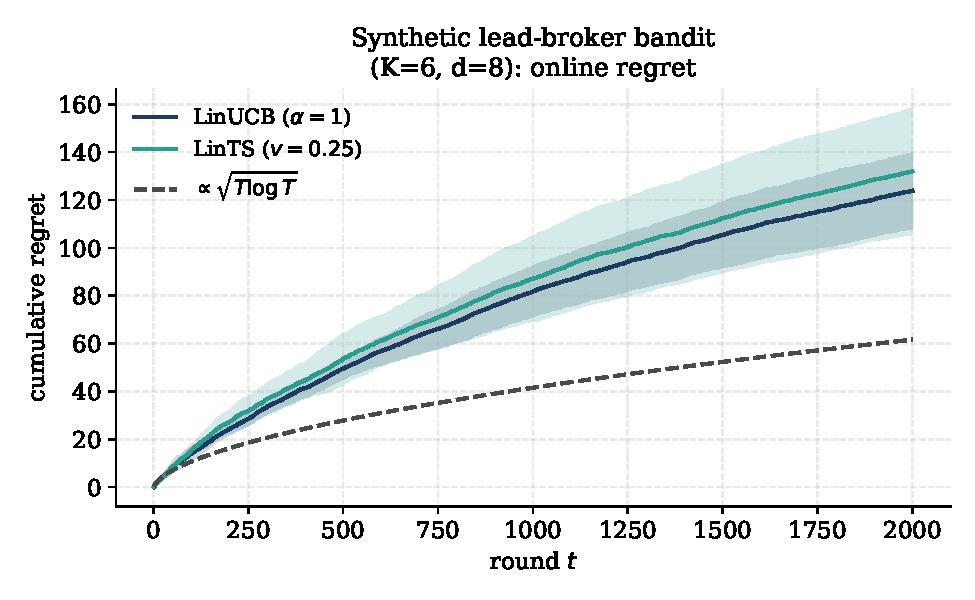
\includegraphics[width=0.88\linewidth]{figs/fig_regret.pdf}
\caption{Cumulative regret on the synthetic insurance lead-broker bandit (4 seeds, mean
$\pm$ std). The dashed reference is $\propto \sqrt{T \log T}$ shape; both
LinUCB and LinTS track it. Random allocation would give a straight line.}
\label{fig:regret}
\end{figure}

\Cref{fig:opebias} compares OPE estimators on the softmax target policy.
IPS has high variance (wide error bar); SNIPS is biased low (the
self-normalisation deflates the estimate when weights are concentrated);
DR sits closest to truth with the smallest variance.

\begin{figure}[h]
\centering
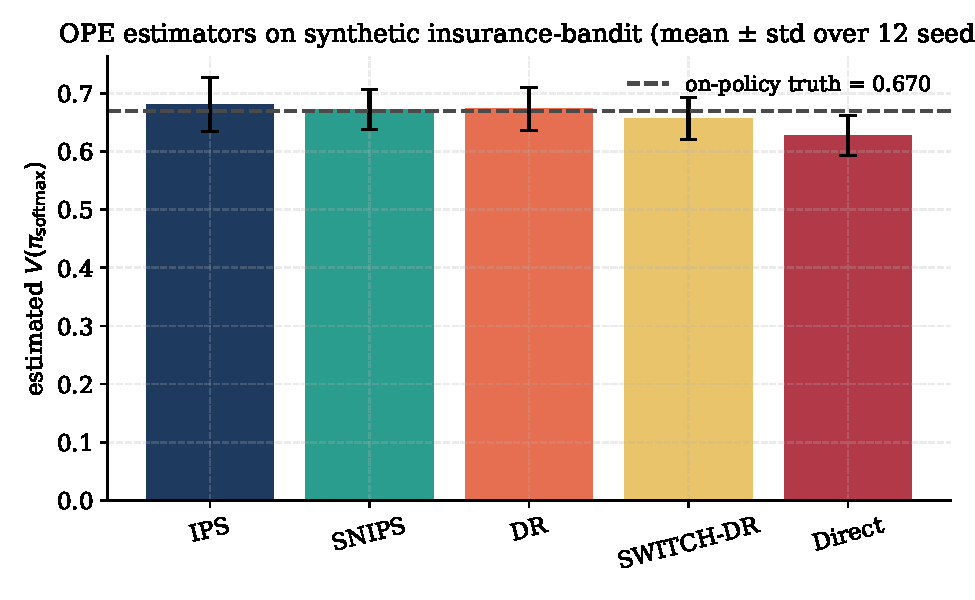
\includegraphics[width=0.88\linewidth]{figs/fig_ope_bias.pdf}
\caption{OPE estimators for a softmax target on the synthetic insurance bandit (12 seeds).
Dashed line is the on-policy ground-truth value computed by Monte Carlo on
fresh contexts.}
\label{fig:opebias}
\end{figure}

\Cref{fig:weights} shows the importance-weight distribution. Under the
oracle-greedy target, a non-trivial fraction of weights exceed $K / \varepsilon
\approx 20$ --- the source of IPS variance.

\begin{figure}[h]
\centering
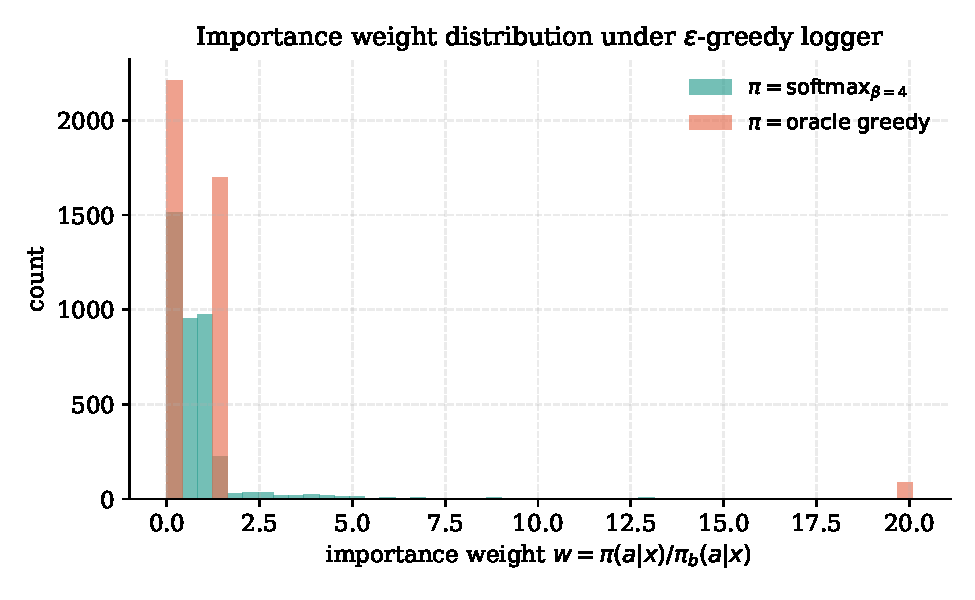
\includegraphics[width=0.85\linewidth]{figs/fig_w_distribution.pdf}
\caption{Importance-weight distribution. The peaky oracle policy puts mass
where $\pi_b$ has $\varepsilon/K$ mass, producing weights of order $20$.}
\label{fig:weights}
\end{figure}

\Cref{fig:bv} shows SWITCH-DR's bias--variance trade-off. Small $\tau$
biases the estimator toward the direct method (low variance, possibly
biased); large $\tau$ recovers pure DR (unbiased, high variance).

\begin{figure}[h]
\centering
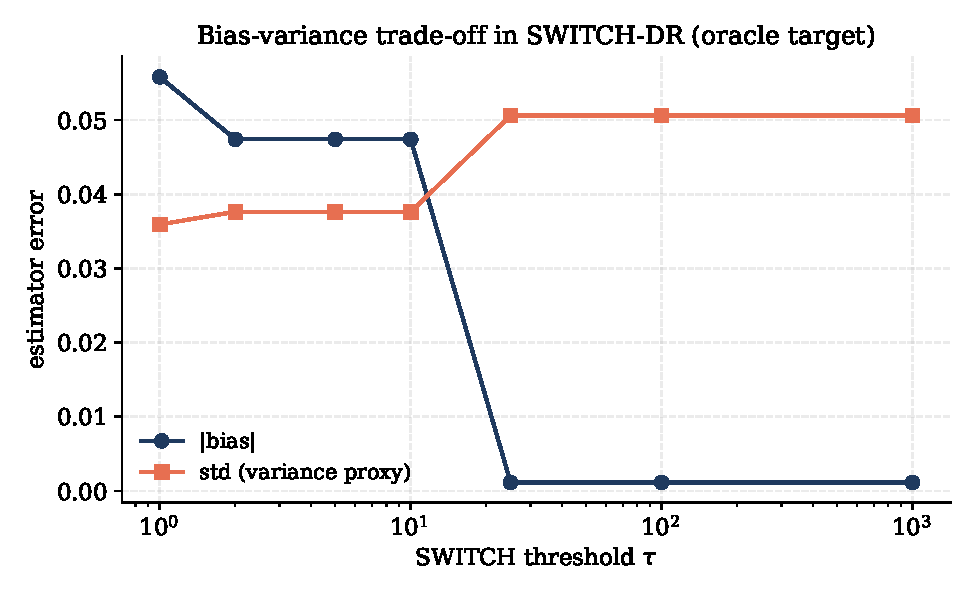
\includegraphics[width=0.88\linewidth]{figs/fig_bias_variance.pdf}
\caption{SWITCH-DR bias and variance vs.\ threshold $\tau$.}
\label{fig:bv}
\end{figure}

% ============================================================================
\chapter{Safety angle}

\begin{safetyangle}
Insurance lead routing is a \emph{high-stakes, delayed-feedback} domain.
Concrete failure modes:

\textbf{F1 --- Naive $\varepsilon$-greedy on real money.} If a broker
specialises in motor and you send them 30\% home-insurance leads ``for
exploration'', you destroy the broker's conversion rate, they raise their
referral fees, and your unit economics collapse. \emph{Mitigation:} cap
$\varepsilon$ per arm using \emph{Conservative Bandits} (Wu, Srikant et al.,
NeurIPS 2016): only explore if a safety constraint
$\hat V(\pi) \geq (1-\zeta) \hat V(\pi_{\mathrm{safe}})$ holds with high
probability.

\textbf{F2 --- IPS with missing propensities.} A common production sin: the
production policy is changed by an engineer, the propensity logger is not
updated, and OPE silently becomes wrong. \emph{Mitigation:} log policy
version hashes alongside the propensity; reject OPE jobs that span a
version boundary.

\textbf{F3 --- Delayed feedback bias.} A lead binds in 1--90 days. If you
evaluate today, recent leads are systematically under-credited. The
estimator is biased \emph{against} new policies (which only have recent
data). \emph{Mitigation:} censor logs to a cooling-off window of at least
the median time-to-bind; or fit a survival model and use predicted-survival
adjusted rewards (Chapelle 2014; Vernade et al.\ 2017).

\textbf{F4 --- Overlap (positivity) failures.} A new broker (cold-start)
has zero historical mass on most leads. Any target policy that prefers them
is un-evaluable by IPS / DR. \emph{Mitigation:} hierarchical Thompson
priors (Kveton et al.\ 2021); explicit cold-start exploration budgets;
honest reporting of ESS (effective sample size).

\textbf{F5 --- Propensity overfitting.} Re-fitting $\pi_b$ from logs leaks
the reward into the propensity, biasing IPS. \emph{Mitigation:} log
propensities at decision time.

Two cites: Bottou et al., \emph{Counterfactual Reasoning and Learning
Systems}, JMLR 2013; Joachims, Swaminathan, de Rijke, \emph{Deep Learning
with Logged Bandit Feedback}, ICLR 2018 (BanditNet).
\end{safetyangle}

% ============================================================================
\chapter{Matching application}

\begin{matching}
The synthetic insurance lead-broker problem is the canonical applied bandit. The mapping:

\begin{center}
\begin{tabular}{lp{0.6\linewidth}}
\toprule
Bandit primitive & synthetic insurance analogue \\
\midrule
context $x$ & lead features (postcode, vehicle, age, channel, prior claims) \\
arm $a$ & broker (one of $K$ panel members) \\
reward $r$ & bind / no-bind (binary) \\
propensity $\pi_b(a|x)$ & probability the production allocator chose broker $a$ for lead $x$ \\
target $\pi$ & candidate policy (re-weighted LinTS, or a fairness-constrained variant) \\
delayed feedback & 1--90 days from quote to bind \\
\bottomrule
\end{tabular}
\end{center}

Engineering implications:
\begin{enumerate}\setlength\itemsep{1pt}
  \item Log $(x, a, r, p, \text{policy\_version\_hash})$ \emph{at decision time}.
  \item Train a calibrated $\hat q(x, a)$ (Beta-calibration on a holdout split).
  \item Run weekly DR + SWITCH evaluations against the next-candidate policy.
  \item Gate deploys behind a conservative bandit bound (Wu et al.\ 2016).
  \item Run a delayed-feedback adjustment (survival head, Chapelle 2014).
\end{enumerate}

A similar mapping works for ATS candidate--job ranking (Week 12), but
position bias and slate structure add a layer of correction.
\end{matching}

% ============================================================================
\chapter{Exercises}

See \texttt{workbook.ipynb} for full statements, hints, and graded tests.
Summary:

\begin{itemize}\setlength\itemsep{2pt}
  \item \textbf{E1} ($\star$) Compute the UCB1 bonus for $t=100$, $n_a=10$.
  \item \textbf{E2} ($\star$) Implement the KL-UCB upper-confidence solver.
  \item \textbf{E3} ($\star\star$) Bernoulli Thompson Sampling on a 3-armed
        bandit; confirm $O(\log T)$ regret growth empirically.
  \item \textbf{E4} ($\star\star$) Train LinUCB on the synthetic insurance bandit; report
        cumulative regret.
  \item \textbf{E5} ($\star\star$) Collect $\varepsilon$-greedy logs; compute
        IPS and SNIPS for a uniform target.
  \item \textbf{E6} ($\star\star$) Doubly Robust against the softmax target;
        compare to the on-policy truth.
  \item \textbf{E7} ($\star$) Effective sample size of importance weights.
  \item \textbf{E8} ($\star\star$) SWITCH-DR; vary $\tau$; observe bias/variance.
  \item \textbf{E9} ($\star\star\star$, \emph{open-ended}, \emph{synthetic insurance objective}) For three counterfactual policies
        (uniform, softmax-true, oracle-greedy) compare SNIPS, DR, and
        SWITCH-DR estimates against on-policy ground truth. Write a one-page
        recommendation memo to the synthetic insurance allocation team.
\end{itemize}

% ============================================================================
\chapter{Further reading}

The \texttt{extended\_reading.pdf} document contains annotated summaries of
five foundational papers: Auer et al.\ 2002 (UCB1), Agrawal \& Goyal 2013
(LinTS), Li et al.\ 2010 (LinUCB), Dud\'ik et al.\ 2011 (DR), Joachims et
al.\ 2018 (BanditNet). For broader context, Lattimore \& Szepesv\'ari,
\emph{Bandit Algorithms} (2020), is the textbook; Bietti, Agarwal,
Langford, \emph{A Contextual Bandit Bake-off} (JMLR 2021) is the empirical
state of the art; and Saito \& Joachims (ICML 2022) introduce MIPS for
large-action OPE --- the natural next step for synthetic insurance / ATS when $K$ grows
from 6 to 6000.

\emph{Sourced from} \texttt{research/bandits\_matching\_sota.md} sections
1--3 (stochastic bandits, contextual bandits, OPE) and
\texttt{research/safety\_rl\_sota.md} (conservative bandits, batch RL safety).

\end{document}
